%%%
%%% expl.tex
%%%


\begin{figure*}[t]
\centerline{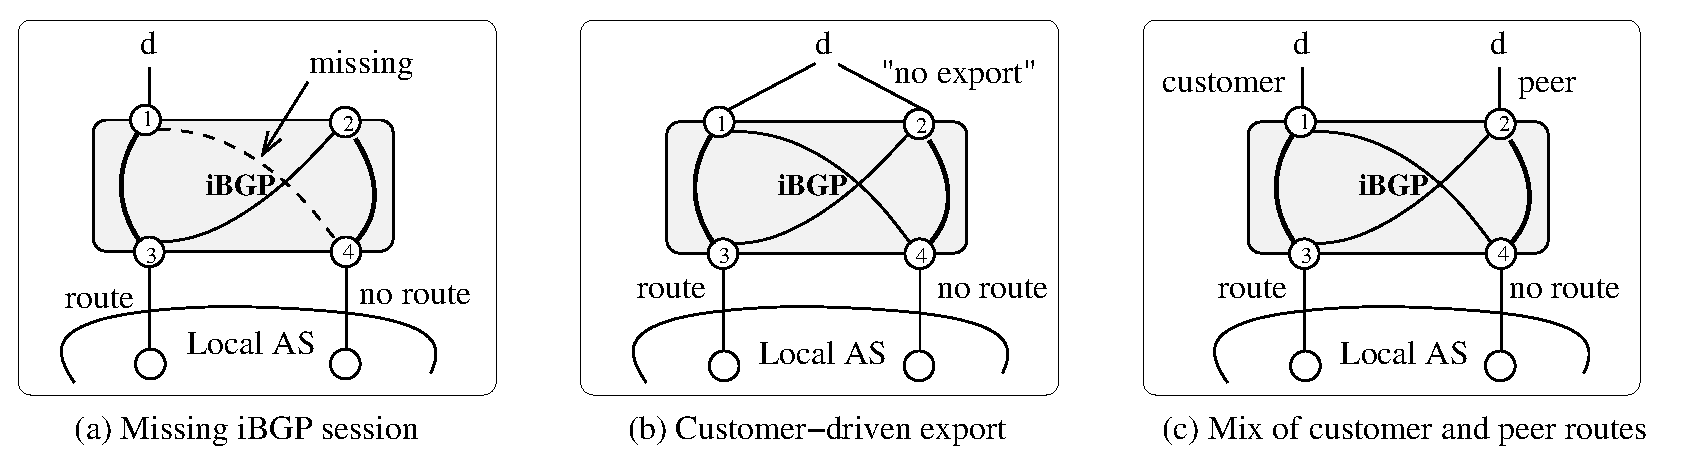
\epsfig{file=dynamic/figures/badpeer.eps,width=\linewidth}}
\caption[Consistent export policies that can lead to inconsistent route export]{Peer AS configurations that lead to inconsistent route export, 
despite consistent export policy.  Router $3$ has a small intradomain
path cost to router $1$, and router $4$ has a small intradomain path
cost to router $2$.}
\label{fig:badpeer}
\end{figure*}

\subsection{How Bad Routes Can Come From Good Peers}
\label{sec:expl}
%%%
%%% Intro
%%%
Although a peer may intentionally violate the ``consistent export''
requirement, inconsistencies may be inadvertent.  For example, a peer
might mistakenly have minor differences in its export policies, such as
filtering small subnets at one location and not another.  However,
applying the {\em same\/} export policy at each peering point does {\em
not\/} guarantee consistent advertisements.  In this subsection, we present
three cases where an AS might not advertise consistent routes to its
peer, even though the AS applies consistent export policies.  Because we
see neither the missing route nor the configuration of the neighboring
AS, we cannot determine what caused the inconsistency (or even whether
it was accidental), but there are at least three plausible explanations
for unintentional inconsistencies:
%In this subsection, we briefly discuss three plausible scenarios that
%would cause a peer to mistakenly advertise inconsistent routes,
%despite having {\em identical\/} export policies at each peering
%point:

\noindent
{\bf Missing iBGP session:} Each router in an AS selects a
single best route for each prefix from the routes learned via iBGP and
eBGP neighbors.  In the simplest scenario, the peer AS has a ``full mesh''
iBGP configuration with a BGP session between each pair of routers.
However, a configuration mistake may lead to a missing iBGP session,
as shown by the dashed line between routers $1$ and $4$ in
Figure~\ref{fig:badpeer}(a).  As a result, router $3$ receives a BGP
route to $d$ but router $4$ does not, leading the peer to advertise
the prefix at one peering point but not the other.  
%A problem like
%this can go undetected because the destination remains reachable.  
A similar configuration mistake could also cause the peer to advertise
routes with different AS path lengths, if one router learns a short
route and another learns a longer route.

Although it might appear that a missing iBGP session is a pathological
case of misconfiguration that would be quickly caught by a network
operator, it turns out that missing iBGP sessions are fairly common, and
can go unnoticed for some time. For example, in
Figure~\ref{fig:badpeer}(a), the destination remains reachable,
so an operator might not immediately notice that router~$4$
does not have complete routing information.  Additionally, larger ASes
often use more complicated iBGP topologies involving route
reflection~\cite{rfc2796}; in these cases, ensuring a fully connected
iBGP topology is more subtle than ensuring a full mesh.  Recent work
that analyzes errors in BGP configuration has discovered that missing
iBGP sessions occur reasonably often~\cite{Feamster2004h}.

\noindent
{\bf Customer-driven export:} Many ASes allow a customer to tag a BGP
route with {\em community\/} attributes that influence the handling of
the route~\cite{rfc1997,rfc1998}.  For example, a customer might be
allowed to use the ``no export'' community~\cite{rfc1997} to instruct
the provider not to export the route to neighboring ASes (\eg, to
control its incoming traffic, the
customer might advertise a subnet of a larger prefix to its immediate
provider but not require that subnet to be propagated further). 
%To control its inbound traffic, a customer could also attach communities
%to certain routes to
%request that its provider  ``prepend'' the AS path for those routes when
%it readvertises them.
%---artificially inflating the length of the
%AS path by repeating the same AS number multiple times---to decrease
%the likelihood that the route is selected by other ASes.  However, the
%customer may not want the prepending to influence its immediate
%provider.  As such, the customer might request (by tagging the route
%with an agreed-upon community) that the provider perform prepending as
%the route is exported to neighboring ASes.  
If the customer connects to the provider in multiple locations, one
route might have this tag and another might not, as shown in
Figure~\ref{fig:badpeer}(b).  The two customer routes look ``equally
good,'' leading routers $3$ and $4$ to select the closest egress point
(routers $1$ and $2$, respectively).  Even if the two routers apply
the same export policy, router $3$ would export the route but router
$4$ would not.  Similarly, an AS might allow its customers to assign
a community that triggers ``AS prepending'' when a route is exported,
which could lead the AS to export routes with different AS path lengths.

\noindent
{\bf Mix of customer and peer routes:} An AS may learn routes for a
prefix from multiple neighboring ASes.  In Figure~\ref{fig:badpeer}(c), 
router $1$ learns a route from a customer and router $2$ learns a
route from a peer.  Suppose the routes have the same AS path length
and that the import policies assign the same local preference to both
routes.  Then, routers $3$ and $4$ would receive two ``equally good''
routes (\ie, with the same local preference and AS path length).
Each router would select the route with the closest egress point,
leading router $3$ to select a customer-learned route and router $4$
to select a peer-learned route.  However, an AS typically does not
export a route learned from one peer to another~\cite{Gao2001a}.  Even
if routers $3$ and $4$ apply exactly the same export policy (\ie,
``export only customer routes''), router $3$ would export a route to
$d$ but router $4$ would not, leading the local AS to receive a route
to the prefix at one peering point and not the other.  We recently
discovered that this very problem was discussed on the North American
Network Operators Group (NANOG) mailing list seven years
ago~\cite{nanog-consistent}. 

Designing tools for detecting these kinds of configuration errors and
policy conflicts would be very useful for preventing unintentional
violations of the ``consistent export'' requirement.

%The example in Figure~\ref{fig:badpeer}(a) arises from a configuration
%mistake that could be caught by the peer AS checking that the iBGP
%session topology is complete~\cite{rcc}.  In contrast,
%Figures~\ref{fig:badpeer}(b) and Figures~\ref{fig:badpeer}(c)
%illustrate interesting ``feature interaction'' problems where two or
%more reasonable goals cannot always be satisfied at the same time.

%In Figure~\ref{fig:badpeer}(b), the peer AS {\em cannot\/} allow
%customers that have multiple connections to request ``prepend on
%export'' while still ensuring consistent export to a neighbor AS.  In
%Figure~\ref{fig:badpeer}(c), the peer AS {\em cannot\/} simultaneously
%assign the same local preference to routes learned from customers and
%peers, selectively export only customer-learned routes to peers, and
%still ensure consistent export at all peering locations.  

\vspace*{-0.1in}
